
%% {
%%     \setbeamercolor{background canvas}{bg=black}
%%     \begin{frame}[plain,c]
%%         \begin{center}
%%         \Huge {\color{white} A quick introduction to Reinforcement Learning}
%%         \end{center}
%%     \end{frame}
%% }

%% * Introduce in a high level what RL is about
%% * Give some examples about its successes 
%% * Give some preliminary hints about the differences to Supervised learning
%% * Give some preliminary hints about what usually can go wrong

\subsection{What is Reinforcement Learning?} \title{What exactly is Reinforcement Learning?} \author{} \date{}
\begin{frame}[plain,c]
    \titlepage
\end{frame}

\begin{frame}
    \frametitle{Reinforcement Learning (RL)}
    \begin{itemize}
        \item A learning approach in which \textbf{agents learn by}
              \textbf{trial and error}.
            \begin{figure}
                \centering
                
\includegraphics[width=0.25\textwidth]{./imgs/img_rl_environment_agent.png}
            \end{figure}
        \pause
        \item A framework for \textbf{sequential} decision making and learning under
              \textbf{uncertainty}.
            \begin{figure}
                \centering
                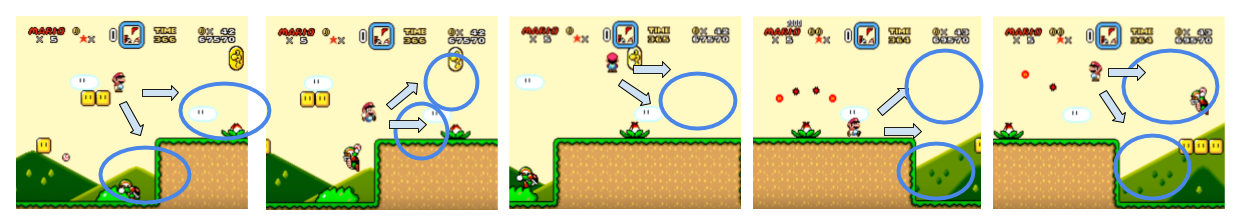
\includegraphics[width=0.9\textwidth]{./imgs/img_sequential_mario.png}
            \end{figure}
    \end{itemize}
\end{frame}

\begin{frame}
    \frametitle{Some RL success stories}
    \begin{figure}[!ht]
        \centering
        \begin{subfigure}{0.4\textwidth}
            \centering
            \href{https://youtu.be/TmPfTpjtdgg}{
\includegraphics[width=0.6\textwidth]{./imgs/img_motivation_dqn_atari.png}}
            \caption{\cite{DQNAtari}}
        \end{subfigure}
        \begin{subfigure}{0.4\textwidth}
            \centering
            \href{https://youtu.be/jGyCsVhtW0M}{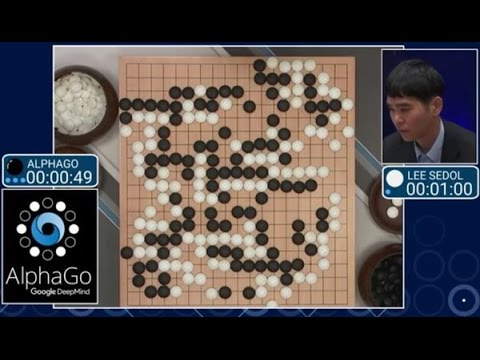
\includegraphics[width=0.7\textwidth]{./imgs/img_motivation_alpha_go.png}}
            \caption{\cite{AlphaGo}}
        \end{subfigure}

        \centering
        \begin{subfigure}{0.4\textwidth}
            \centering
            \href{https://youtu.be/hx_bgoTF7bs}{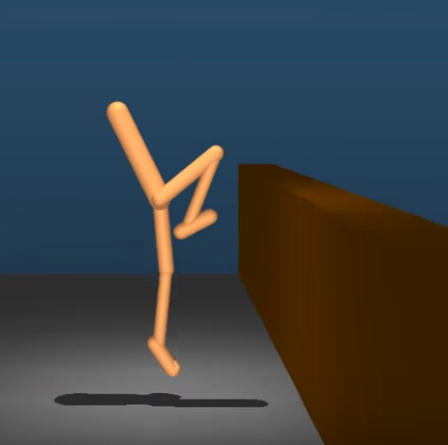
\includegraphics[width=0.6\textwidth]{./imgs/img_motivation_locomotion.png}}
            \caption{\cite{DeepmindEmergenceLocomotion}}
        \end{subfigure}
        \begin{subfigure}{0.4\textwidth}
            \centering
            \href{https://youtu.be/vppFvq2quQ0}{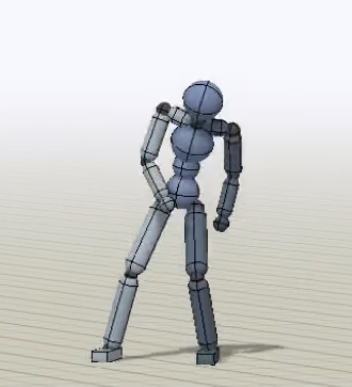
\includegraphics[width=0.6\textwidth]{./imgs/img_motivation_deepmimic.png}}
            \caption{\cite{DeepMimic}}
        \end{subfigure}
    \end{figure}
\end{frame}